%!TEX root=bare_conf.tex
\section{Evaluation}\label{sec:evaluation}

In general, this paper investigates the following research questions to evaluate PML\_Checker:
\begin{description}
\item[RQ1:] How does our approach perform under the public benchmarks in terms of accuracy and efficiency analysis? 
\item[RQ2:] How does our approach perform in terms of effectiveness analysis for complex control flows? 
\item[RQ3:] How does our approach perform in terms of effectiveness analysis for complex data types? 
\end{description}

\subsection{Evaluation on public benchmarks}

\noindent RQ1: \textit{Accuracy and Efficiency of PML\_Checker}
%The first research question is to compare the accuracy achieved by the four approaches, and the run-time recorded by the corresponding $4$ tools in terms of open benchmarks. There are two experiments.

\subsubsection{Accuracy Analysis} 

This experiment analyzed the test results and run time of the four tools on SPEC CPU $2000$ and SIR, and the \textit{FP} was selected to measure the accuracy of different approaches on the same test suite. Table~\ref{tab:4} shows the test results on SPEC CPU $2000$ and Table~\ref{tab:5} shows the test results on SIR. Compare our approach with other approaches, we have the following observations. 
%First, we calculate the false positive rates in Table~\ref{tab:4}, i.e., \textit{FP}(CppCheck) =$ 2/19$ $\approx$ 0.11. \textit{FP}(Splint) = 0.44. \textit{FP}(RL\_Detector) = 0.09. \textit{FP}(PML\_Checker) = 0.13. Similarly, in Table~\ref{tab:5}, \textit{FP}(CppCheck) = 0.19, \textit{FP}(Splint) = 0.30, \textit{FP}(RL\_Detector) = 0.08, \textit{FP}(PML\_Checker) = 0.18.

\begin{table}[!h]
\centering
\setlength{\abovecaptionskip}{0pt}%    
\setlength{\belowcaptionskip}{10pt}%
\caption{Test results on SPEC CPU $2000$}\label{tab:4}
\centering
\begin{tabular}{|c|c|c|c|c|c|c|c|c|c|}
\hline
&  & \multicolumn{2}{|c|}{\textbf\small{CppCheck}} & \multicolumn{2}{|c|}{\textbf\small{Splint}} &          \multicolumn{2}{|c|}{\textbf\small{RLDetector}} & \multicolumn{2}{|c|}{\textbf\small{PMLChecker}}\\
\hline
\textbf\small{Program} & \textbf\small{Kloc} & \textbf\small{TW} & \textbf\small{NF} & \textbf\small{TW} & \textbf\small{NF} & \textbf\small{TW} &   \textbf\small{NF} & \textbf\small{TW} & \textbf\small{NF}\\
\hline
gzip       & 7.8    & 1  & 1 & 1	& 1   & 1   & 1  & 3  & 1\\
\hline
vpr        & 17.0   & 0  & 0 & 0	 & 0   & 0  &	0  &	4   &1\\
\hline
gcc        & 205.8 & 1  & 0 & 46 & 24 & 35 &	0  & 22 & 1\\
\hline
mesa     & 49.7   & 1  & 0 & 9	 & 5	   & 4  & 2  & 17 & 5\\
\hline
art         & 1.3     & 1  & 0 &0   & 0	   & 1  &	0   & 3  & 0\\
\hline
mcf        & 1.9     & 0  & 0 & 5  &  2  & 0   & 0  & 1  & 1\\
\hline
equake   & 1.5     & 0  & 0 & 0	 & 0   &	0  & 0   & 8  & 0\\
\hline
crafty     & 18.9   & 0	 & 0	 & 0	 & 0	  & 0   & 0   & 0   & 0\\
\hline
ammp    & 13.3   & 12 & 0 & 22 & 4  & 	20 & 0  & 22 & 2\\
\hline
parser    & 10.9   & 0	 & 0	 & 0	   &0  & 0    & 0  & 0  & 0\\
\hline
perlbmk & 58.2   & 2   & 1	 & 0	   & 0  &	4   & 1  & 2  & 0\\
\hline
gap        & 59.5   &  0 & 0 & 0    & 	0  &	0   & 0   & 0	& 0\\
\hline
vortex    & 52.7    & 0	 & 0	 & 0	   & 0  &	0   & 0   & 0	& 0\\
\hline 
bzip2     & 4.6      & 1 & 0	 & 2	   & 1  &	0   & 0   & 1	& 0\\
\hline
twolf     & 19.7     & 0 & 0	 & 0	   & 0  &	0   & 0   & 0	& 0\\
\hline
Total     & 581      & 19 & 2 & 85 &	37 & 65 & 6	& 83 & 11\\
\hline
\multicolumn{2}{|c|}{FP} & \multicolumn{2}{|c|}{11\%} & \multicolumn{2}{|c|}{44\%} & \multicolumn{2}{|c|}{9\%}  &\multicolumn{2}{|c|}{13\%}\\
\hline
\end{tabular}
\end{table}

\begin{table}[!h]
\centering
\setlength{\abovecaptionskip}{0pt}%    
\setlength{\belowcaptionskip}{10pt}%
\caption{Test results on SIR}\label{tab:5}
\centering
\begin{tabular}{|c|c|c|c|c|c|c|c|c|c|}
\hline
&  & \multicolumn{2}{|c|}{\textbf\small{CppCheck}} & \multicolumn{2}{|c|}{\textbf\small{Splint}} &           \multicolumn{2}{|c|}{\textbf\small{RLDetector}} & \multicolumn{2}{|c|}{\textbf\small{PMLChecker}}\\
\hline
\textbf\small{Program} & \textbf\small{Kloc} & \textbf\small{TW} & \textbf\small{NF} & \textbf\small{TW} & \textbf\small{NF} & \textbf\small{TW} & \textbf\small{NF} & \textbf\small{TW} & \textbf\small{NF}\\
\hline
bash       & 59.8 &7	&1	  & 15  & 3  & 3	 & 0   & 17  & 2\\
\hline
flex	       & 10.5  & 1	& 0	  & 2    & 1  & 2	 & 1	   & 2   & 1\\
\hline
grep	 & 10.1 & 3	& 1	  & 0    & 0  & 0	 & 0	   & 2   & 0\\
\hline
gzip	       & 5.7   & 0	& 0	  & 0    & 0  & 0	 & 0	   & 0   & 0\\
\hline
make	 & 35.5 &1	& 0	  & 0    & 0  & 0	 & 0	   & 1   & 0\\
\hline
print	 & 0.7   &  0	& 0	  & 0    & 0  & 0	 & 0	   & 0   & 0\\
\hline
print2	 & 0.6   & 0	& 0	  & 0    & 0  & 0	 & 0   &	0   & 0\\
\hline
replace    & 0.6   & 0	& 0	  & 0    & 0  & 0	 & 0	   & 0   & 0\\
\hline
schedule  & 0.4	& 0	& 0	  & 5    & 2  & 0	 & 0	   & 2   & 0\\
\hline
schedule2 & 0.4	& 0	& 0    & 3    & 0  & 0	 & 0	   & 2   & 1\\
\hline
sed	        & 14.4	& 4	& 2    &	0   & 0  & 0	 & 0	   & 3   & 0\\
\hline
space	 & 6.2	& 2	& 0	   & 0   & 0  & 0	 & 0	   & 1   & 1\\
\hline
tcas	       & 0.2	& 0	& 0    &	0   & 0  & 0	 & 0    & 0   & 0\\
\hline
totinfo	 & 0.6	& 0  & 0	   & 0    & 0  & 0	 & 0	   & 0   & 0\\
\hline
vim        & 122.2	& 3	& 0	   & 12  & 5  & 8	 & 0	   & 4   & 1\\
\hline
Total	 & 267.9	 & 21&4	   & 37  & 11 & 13 & 1   & 34  & 6\\
\hline
\multicolumn{2}{|c|}{FP} & \multicolumn{2}{|c|}{19\%} & \multicolumn{2}{|c|}{30\%} & \multicolumn{2}{|c|}{8\%} & \multicolumn{2}{|c|}{18\%}\\
\hline
\end{tabular}
\end{table}
First, in the view of \textit{TW} from Table~\ref{tab:4} and Table~\ref{tab:5}, Splint reported most bugs, and PML\_Checker ranked second, while CppCheck reported the least bugs. However, in the view of \textit{NF}, the \textit{FP} of Splint is the highest, and the \textit{FP} of the other three tools are acceptable.

Second, this paper analyzes the effectiveness of the CFG projection approach by comparing the MLF of test results. The table of test  results is converted into MLF of test results by constructing a matrix. The results from Table~\ref{tab:4} can be abstracted to a sparse matrix consists of $15$ quaternions. This paper compress this matrix by removing all the rows that test results are zero, and a row in the matrix corresponds to a row in the table of test results, the final matrix $D_1$ is as follows.
\[
\scriptsize
D_1=\left[
\begin{array}{cccccccccc}
0 & 0 & 35 & 2 & 1 & 0 & 0 & 20 & 3 & 0\\
0 & 0 & 1  &  1 & 1 & 0 & 0 & 12 & 1 & 1\\
0 & 0 & 22 & 4 & 0 & 3 & 0 & 18 & 0 & 1 \\
2 & 3 & 21 & 12 & 3& 0 & 8 & 20 & 2 & 1  
\end{array}
\right]^{T}
\]

$D_2$ is the matrix abstracted from Table~\ref{tab:5}, and $D_2$ is shown as follow:
\[
\scriptsize
D_2=\left[
\begin{array}{ccccccccc}
3 & 1 & 0 & 0 & 0 & 0 & 0 & 0 & 8 \\
6 & 1 & 2 &  1 & 0 & 0 & 2 & 2 & 3\\
12 & 1 & 0 & 0 & 3 & 3 & 0 & 0 & 7 \\
15 & 1 & 2& 1 & 2 & 1 & 3 & 0 & 3  
\end{array}
\right]^{T}
\]

\begin{figure}[!h]
\center
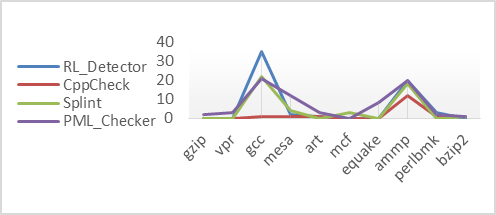
\includegraphics[width=0.45\textwidth]{figure/fig8-fig12/fig10}
\caption{The MLF of each tool on SPEC CPU 2000}
\label{fig:10}
\end{figure}

\begin{figure}[!h]
\center
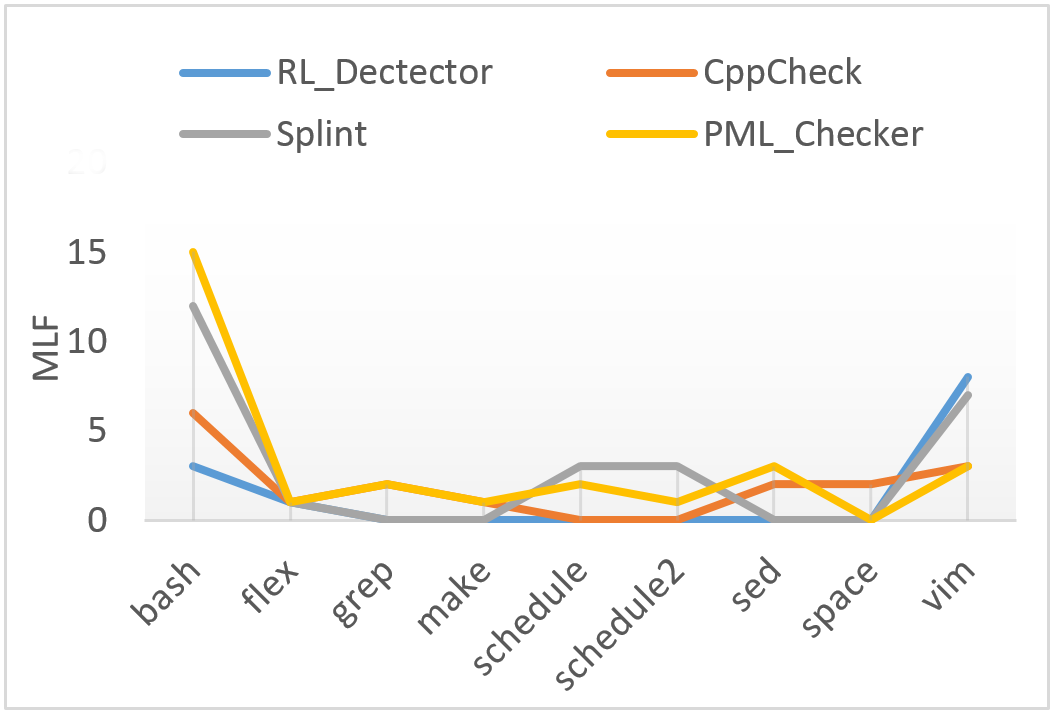
\includegraphics[width=0.45\textwidth]{figure/fig8-fig12/fig11}
\caption{The MLF of each tool on SIR}
\label{fig:11}
\end{figure}

In Fig.~\ref{fig:10}, the abscissa shows the name of the program corresponding to each row in the matrix, the ordinate shows the value of corresponding MLF. This figure displays the number of memory leaks confirmed by manually checking, among the test results on the $15$ programs from SPEC CPU $2000$. We conclude from the figure that the CFG projection has a good detection result on all the test sets except gcc, for the reasons that the program gcc is larger than others in scale. Therefore, we deduce that the scalability of the CFG projection approach for large scale test objects needs to be improved. While in Fig.~\ref{fig:11}, due to the smaller amount of loc(line of code) comparing to SPEC CPU 2000 and fewer \textit{TW} of each tool, the advantage of PML\_Checker is not obvious. But the analysis results between the two benchmarks are generally consistent.


\noindent\textbf{Experiment on test cases from SARD} 
\\
This experiment analyzed the results of the four tools on test cases from SARD. The \textit{FP} and \textit{NP} were measured to the accuracy of different approaches on the same test suite. Table~\ref{tab:7} shows the test results on these test cases, and Fig.~\ref{fig:12} is a histogram that compares test results metrics of the four detection tools. Comparing our approach with other approaches, we have the following observations.

%First, we calculated the false negative rate from the test results of $20$ test cases with memory errors marked ``bad", and the false positive rate from the test results of $20$ test cases without memory errors which corresponding to the ``bad" cases marked ``good". Specifically, \textit{NP}(RL\_Detector) = 0.7, and \textit{FP}(RL\_Detector) = 0. \textit{NP}(CppCheck) = 0.5, and \textit{FP} (CppCheck) = 0. \textit{NP}(Splint) = 0.8, and \textit{FP}(Splint) = 0.05. \textit{NP}(PML\_Checker) = 0.3, and \textit{FP}(PML\_Checker) = 0.

The \textit{FP} of PML\_Checker is the lowest among the four tools. For the analysis of \textit{FP}, there are no false positives in the results of RL\_Detector, CppCheck and PML\_Checker, while Splint reported a false positive, which confirmed that Splint has a high \textit{FP} in experiment \RNum{1}. This experiment failed to compare the \textit{FP} due to the small scale of the programs, but the test results on \textit{NP} reflected the accuracy of our approach in detecting memory leaks.

\begin{table}[!h]
\center
\caption{Test results on SARD test cases}\label{tab:7}
\begin{tabular}{|c|c|c|c|c|}
\hline
\textbf{Test Cases} & \textbf{A1} (TW)& \textbf{A2} (TW) & \textbf{A3} (TW) & \textbf{A4} (TW)\\
\hline
bad cases(20) &10 & 4 & 6 & 14\\
\hline
good cases(20) & 0 & 	1 &	0 &	0\\
\hline
FP & 0& 5\% & 0 & 0\\
\hline
NP & 50\% & 80\% & 70\% & 30\%\\
\hline
\end{tabular}
\end{table}

%\begin{figure}[!h]
%\center
%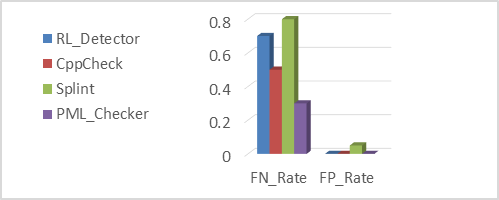
\includegraphics[width=0.45\textwidth]{figure/fig8-fig12/fig12}
%\caption{The bar chart of test results}
%\label{fig:12}
%\end{figure}

\subsubsection{Efficiency Analysis} 

Considering symbolic method are used in CppCheck, RL\_Detector and PML\_Checker, meanwhile, in order to verify whether our approach to influence the running time, so this section chooses SPEC CPU 2000 as the test object due to its large amount of code and large number of files, compared and analyzed run time of the three tools.  Table~\ref{tab:6} lists the run-time on this benchmark. Comparing the run-time of these three tools, we conclude that the performance of RL\_Detector and PML\_Checker is better than CppCheck in run-time, and our approach did not affect the run time of PML\_Checker.

\begin{table}[!h]
\centering
\caption{Run time on SPEC CPU $2000$}\label{tab:6}
\centering
\begin{tabular}{|c|c|c|c|c|}
\hline
\textbf{Program}& \textbf{Size} & \textbf{CppCheck} & \textbf{RL\_Detector} & \textbf{PML\_Checker}\\
\hline
gzip       & 7.8    & 5.3s  & 4.5s & 3.2s\\
\hline
vpr        & 17.0   & 10.0s  & 7.5s & 7.6s\\
\hline
gcc        & 205.8 & 167.7s  & 48.3s & 41.0s \\
\hline
mesa     & 49.7   & 51.0s  & 33.1s & 34.8s\\
\hline
art         & 1.3     & 0.3s  & 0.9s & 0.4s\\
\hline
mcf        & 1.9     & 1.0s  & 4.0s & 3.7s\\
\hline
equake   & 1.5     & 0.2s  & 1.0s & 0.4s\\
\hline
crafty     & 18.9   & 27.3s	 & 14.2s	 & 13.3s\\
\hline
ammp    & 13.3   & 7.4s & 10.3s & 10.0s\\
\hline
parser    & 10.9   & 4.0s	 & 6.7s	 & 5.1s\\
\hline
perlbmk & 58.2   & 123.2s   & 41.3s	 & 39.0s\\
\hline
gap        & 59.5   &  29.0s & 20.9s & 20.0s\\
\hline
vortex    & 52.7    & 73.2s	 & 30.1s	 & 26.7s\\
\hline 
bzip2     & 4.6      & 2.0s & 0.6s	 & 1.5s\\
\hline
twolf     & 19.7     & 11.0s & 23.7s	 & 24.0s\\
\hline
Total     & 581.0    & 512.6s & 247.1s & 230.7s\\
\hline
\end{tabular}
\end{table}

\subsection{Evaluation on Study Cases}

\noindent RQ2: \textit{Effectiveness Analysis of Complex Control Flows}

\begin{table}[!h]
\center
\caption{Test results on complex control flows}\label{tab:2}
\begin{tabular}{|c|c|c|c|c|}
\hline
\textbf{No.}  & \textbf{CppCheck} & \textbf{Splint} & \textbf{RL\_Detector} & \textbf{PML\_Checker}\\
\hline
1	 &	YES & NO & YES & YES\\
\hline
%C\_case2 & Simple\_branch\_2 & \textendash & \textendash & \textendash & \textendash\\
%\hline
2	 & NO &	NO & YES & YES\\
\hline
3    & YES & NO & YES & YES\\
\hline
4	 & NO & NO & YES & YES\\
\hline
5	 &	NO	& NO & YES & YES\\
\hline
6	 & YES & YES & NO & YES\\
\hline
7	 & YES& YES & NO & YES\\
\hline
8	 & NO & NO & YES & YES\\
\hline
9 & NO & NO & YES & YES\\
\hline
NP & 56\% & 78\% & 22\% & 0\\
\hline
\end{tabular}
\end{table}

%\begin{figure}
%\center
%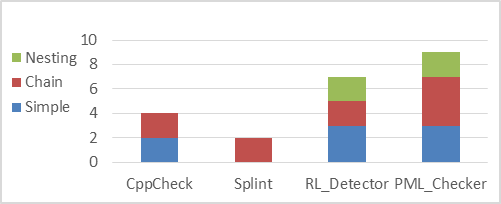
\includegraphics[width=0.45\textwidth]{figure/fig8-fig12/fig8}
%\caption{Description of memory leaks reasons}
%\label{fig:8}
%\end{figure}

%First, all the $4$ tools did not detect the memory leak in C\_case2, because the memory leaks in C\_case2 are caused by allocating memory blocks in conditional branches. In this case, the program will be compiled failed, because the pointer pointing to memory blocks is not found during the execution of function ``free()". Therefore, this type of test case is often ignored in static analysis.

%First, we calculated the \textit{NP} of the test results. In details, the false negative rate of CppCheck test results, that is \textit{NP}(CppCheck) is 5/9 $\approx$ 0.56. In the same way, \textit{NP}(Splint) = 0.78, \textit{NP}(RL\_Detector) = 0.22, while \textit{NP}(PML\_Checker) = 0. For the reason that the analysis method of PML\_Checker is based on the complex control flow, the results of PML\_Checker covered all the test cases about complex control flow in this experiment. In other words, the false negative rate of the CFG projection approach is lower than other approaches for detecting memory leaks in complex control flow, which reflects the effectiveness of this approach for complex control flow.
Table~\ref{tab:2} lists the test results on $10$ small programs. Comparing our approach to three other approaches, we have the following observations.
First, PML\_Checker covered all the test cases about complex control flow in this experiment. In other words, the \textit{NP} of the CFG projection approach is lower than other approaches for detecting memory leaks in complex control flow, which reflects the effectiveness of this approach for complex control flow.
Second, regarding the comparison of the approaches, the regular match based approach compares the source code with the vulnerabilities in the process of detecting memory leaks. This approach is not sensitive to complex control flow and inflexible in the types of vulnerabilities to compare with. The style and notation based approach improves the software quality by improving the programming style and discovering the potential bugs that impacting the portability of programs. However, the memory leak analysis is not complete, so it has a high false negative rate. The approach by constructing resources streamlined slices only makes a simple assumption for allocation and deallocation of resources within loop bodies. It reduces the number of loops to 1 and treats the loops the same as branches. Therefore, this approach can not pass the test cases on the Chain\_Loop structure (C\_case6 and C\_case7) in the experiment.\\


\noindent RQ3: \textit{Effectiveness Analysis of Complex Data Types}

\begin{table}[!h]
\center
\caption{Test results on complex data types}\label{tab:3}
\begin{tabular}{|c|c|c|c|c|}
\hline
\textbf{No.}  & \textbf{CppCheck} & \textbf{Splint} & \textbf{RL\_Detector} & \textbf{PML\_Checker}\\
\hline
1	 &	YES & NO & YES & YES\\
\hline
2  & NO & NO & NO & NO \\
\hline
3	 & NO &	NO & NO & YES\\
\hline
4		& NO &	NO & NO & NO\\
\hline
5	 & NO & YES & NO & YES\\
\hline
6	 &	NO	& YES & NO & YES\\
\hline
7	 & NO & YES & NO & YES\\
\hline
8	 & NO & YES & NO & YES\\
\hline
9	 & NO & YES & YES & YES\\
\hline
10  & YES & YES & YES & YES\\
\hline
NP & 80\% & 40\% & 70\% & 20\%\\
\hline
\end{tabular}
\end{table}

%\begin{figure}[!h]
%\center
%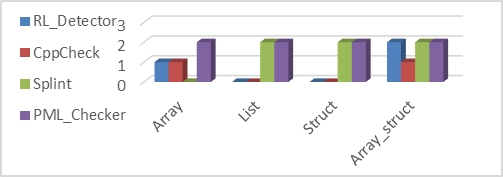
\includegraphics[width=0.45\textwidth]{figure/fig8-fig12/fig9}
%\caption{The leaks number of each data type}
%\label{fig:9}
%\end{figure}

%First, the common high NP shows us the accuracy of pointer alias analysis on complex data flow is relatively lower for all the tools.
Table~\ref{tab:3} lists the test results on $10$ small programs. Comparing our approach with other approaches, we have the following observations.

First, the results of Splint and PML\_Checker show a higher effectiveness compared with the other two tools in the experiment. Splint has a high effectiveness because it mainly checks the specifications in programs, which is sensitive to different data types. Splint has a high effectiveness because it simplifies the analysis for complex data types in the process of abstracting the control flows. 
Second, comparing PML\_Checker with Splint, Splint reported memory leaks on the latter three data types (linked list, struct and array\_struct), except the memory leaks in an array. Due to the programs that are provided in this paper are in small scale and simple data relationships, PML\_Checker shows a little advantage compared to Splint. For the former approaches, that is CppCheck and RL\_Detector, there is a large space to improve in analyzing the complex data types.

\subsection{Summary}
From the above experimental results, we have the following main findings including advantages and limitations: 
\begin{itemize}
\item 
For the complex control flows and complex data types analysis, our projection-based approach is better than the other three approaches.
\item 
For the accuracy of detection, our projection-based approach shows a lower false negative rate compared to other tools, while it shows a high false positive rate in some public benchmarks (such as SPEC CPU $2000$ and SIR). Therefore, in the next step, more detailed data flow analysis will be added into our approach.
\item 
For the scalability of detection, our experiment needs to expand the range of detection. Specifically, our system will detect the large scale benchmarks with millions of code lines, or source code from some open-source software.
\end{itemize}
